% F089｜勾股整数数组的构造规律｜06_summary.tex
% 继承上传模板的 LaTeX 环境；当前条目的内容独立编写。
\clearpage
\begin{summarybox}
\textbf{\textcolor{CSummary}{快记、快懂、快用}}
\par\medskip
\begin{center}
% F089｜formula 原创简明教学示意图
\begin{tikzpicture}[>=stealth,scale=.9]
\node[draw,rounded corners,fill=teal!9] (a) at (0,0) {$m>n>0$};
\node[draw,rounded corners,fill=orange!10] (b) at (4.5,0) {$m^2-n^2,\ 2mn,\ m^2+n^2$};
\draw[->,thick] (a)--(b);
\node at (4.5,-1){\small 任取正整数 $m>n$，都会得到一组勾股数};
\end{tikzpicture}

\end{center}
\medskip
\textbf{快记：}$m^2-n^2,2mn,m^2+n^2$。\par\textbf{快懂：}展开后两边平方和恒等于斜边平方。\par\textbf{快用：}要“造一组”用 F089；要“找全组”用 F090。
\end{summarybox}
\clearpage
\begin{summarybox}
\textbf{\textcolor{CSummary}{奇偶直角边一眼记}}
\par\medskip
\begin{center}
% F089｜odd 原创简明教学示意图
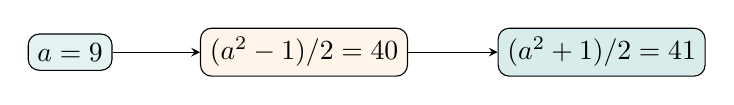
\begin{tikzpicture}[>=stealth,scale=.9]
\node[draw,fill=teal!10,rounded corners] (a) at (0,0){$a=9$};
\node[draw,fill=orange!8,rounded corners] (b) at (3.3,0){$(a^2-1)/2=40$};
\node[draw,fill=teal!15,rounded corners] (c) at (7.5,0){$(a^2+1)/2=41$};
\draw[->] (a)--(b);\draw[->] (b)--(c);
\end{tikzpicture}

\end{center}
\medskip
\textbf{奇数：}先平方，再一减一加后都除2。\par\textbf{偶数：}先取一半，再平方，最后减1和加1。\par\textbf{检查：}直角边都大于0，结果确为整数。
\end{summarybox}
